\documentclass[a4paper,10pt,twoside]{article}
\usepackage{amsmath}
\usepackage{its_conf}

\begin{document}
\setcounter{section}{0}
\setcounter{figure}{0}
\setcounter{table}{0}
\setcounter{equation}{0}
\setcounter{secnumdepth}{1}

% ======= Title, author, abstract =======

\topic{Non-Stationarity of Long-Term Memory in Financial Volatility and Its Predictive Value: Empirical Evidence and Implications for Memory-Adaptive Attention in Transformers}

\information{Bondarenko~D.~D.}
{Department of Probability Theory and Mathematical Statistics, Belarusian State University}
{Minsk, Republic of Belarus}{adarka.bon@gmail.com}

\annotation{Volatility forecasting is a core problem of modern financial analysis: the accuracy of
volatility models directly determines the quality of market-risk measures, capital allocation and
derivative pricing. Financial volatility is known to exhibit long-term memory --- the slow,
power-law decay of the autocorrelation function --- and this effect underlies the FIGARCH,
ARFIMA-RV and HAR-RV model families. A growing body of evidence, however, indicates that the
\emph{strength} of this memory is not a constant characteristic of the process but a dynamic,
regime-dependent property that weakens in crisis periods. Existing deep-learning architectures do
not exploit this fact: the self-attention mechanism of the Transformer behaves as a learnable
autocorrelation function, yet the attention schemes of Informer, Autoformer and PatchTST are
specified a priori and therefore do not follow the current memory regime. Using daily data for ten
assets (five stocks, two cryptocurrencies and three currency pairs) over 2019--2023, we estimate the
local memory of realized volatility by means of the rescaled-range analysis and the
Geweke--Porter-Hudak estimator in a rolling window of 500 observations, and test for structural
breaks in the resulting trajectories with a CUSUM test. The local memory parameter $d$ of realized
volatility is found to be significantly non-stationary for seven of the ten assets, and to collapse
during crises (the mean value falls from $0.52$ to $0.45$). Adding the local memory estimate and its
first difference to HAR-RV improves the mean-squared error for all ten assets (on average by
$+7.1\%$) and the QLIKE loss for eight of ten (on average by $+1.8\%$). A pilot experiment on
minute-frequency quotes shows that the static attention mechanisms Standard, ProbSparse and
MultiFeature degrade by $+51\%$, $+143\%$ and $+50\%$ in RMSE respectively when the memory regime
switches. On this basis we formulate the Memory-Adaptive Attention mechanism, in which a
differentiable local memory estimator acts as a control signal that adapts the context length and
the sparsity of attention to the current memory regime, and we outline the corresponding VaR/ES
backtesting programme.}

\textbf{Keywords:} long-term memory, realized volatility, non-stationarity, Hurst exponent,
Geweke--Porter-Hudak estimator, HAR-RV, transformer, self-attention, volatility forecasting,
Value-at-Risk.

\begin{multicols}{2}

% ======= 1. Introduction =======

\section{Introduction}

\subsection{Motivation}

Volatility --- a measure of the intensity of price fluctuations of a financial asset --- is a key
object of study in financial economics. The accuracy of volatility forecasts determines the
precision of risk measures (Value-at-Risk and Expected Shortfall), the capital that has to be
allocated against market risk, the pricing of derivative instruments and the construction of
efficient portfolios. Over the last three decades the modelling of volatility has followed a
clearly traceable path: from conditional heteroskedasticity models of the GARCH family and their
fractionally integrated generalisations to realised volatility models such as HAR-RV, and from there
to deep learning architectures in which the attention mechanism replaces explicit multi-scale
autoregressive structure.

Two features of volatility have shaped this development. The first is \emph{long memory}: the
autocorrelation function of volatility decays hyperbolically rather than exponentially, so that
observations hundreds of steps away retain statistically significant influence on the current
dynamics. The second, and far less exploited, feature is that the \emph{strength} of this memory
changes over time. Empirical studies report that the persistence of volatility is systematically
lower in turbulent periods than in calm ones. A model that treats the memory structure as fixed is
therefore mis-specified precisely in the periods in which the consequences of mis-specification are
most costly.

\subsection{The research problem and the questions addressed}

The problem addressed in this paper is formulated as follows. \textbf{Research problem:} the
strength of long-term memory in the volatility of financial time series is a non-stationary,
regime-dependent property; models that impose a fixed memory structure --- both the classical
econometric families and the current Transformer-based forecasters --- are therefore systematically
mis-specified at regime changes, and a mechanism that adapts to the locally estimated memory is
required.

Three questions are addressed empirically:

\begin{itemize}
\item \textbf{Q1.} Is long-term memory in financial volatility genuinely non-stationary, and can
the change be tied to identifiable market regimes?
\item \textbf{Q2.} Does the \emph{local} estimate of the memory parameter carry predictive
information about future volatility that is not already contained in the standard HAR-RV
specification?
\item \textbf{Q3.} Do existing static attention mechanisms degrade differently across memory
regimes, which would motivate an adaptive alternative?
\end{itemize}

\subsection{Contributions}

The contribution of the paper is threefold. First, it provides a systematic empirical
demonstration that long-term memory in realised volatility is non-stationary across a
heterogeneous cross-section of ten assets from three asset classes, and that the weakening of
memory is regime-linked rather than asset-specific. Second, it establishes that the local memory
estimate carries independent forecasting content, quantified through a controlled comparison
against HAR-RV. Third, it translates the statistical evidence into a machine-learning design
principle: since self-attention constitutes a learnable autocorrelation function, an attention
scheme that is fixed a priori cannot be optimal across regimes, and a Memory-Adaptive Attention
mechanism driven by a differentiable memory estimator is proposed as the corresponding remedy.

\subsection{Organisation of the paper}

Section~\ref{sec:related} reviews the literature on long memory in volatility, on econometric
long-memory models, and on Transformer architectures for time series forecasting. Section
\ref{sec:data} describes the data. Section~\ref{sec:method} presents the estimation of the local
memory parameter, the testing procedure for non-stationarity, the forecasting experiment and the
attention experiment, and formulates the Memory-Adaptive Attention mechanism. Section
\ref{sec:results} reports the results, and Section~\ref{sec:discussion} discusses them, including
the important caveat raised by recent work on the estimation of long memory. Section
\ref{sec:concl} concludes.

% ======= 2. Related work =======

\section{Related work}\label{sec:related}

\subsection{Long memory in financial volatility}

The observation that volatility is more persistent than returns goes back to the seminal analyses of
Ding, Granger and Engle [11] and of Andersen, Bollerslev, Diebold and Labys
[1]. The canonical characterisation is that the autocorrelation function
of volatility decays as a power law, which is captured by the fractional differencing operator
$(1-L)^d$ with $d\in(0,1/2)$; in the Brownian-motion parameterisation the relation
$d=H-1/2$ links the fractional integration order to the Hurst exponent $H$ [16, 21]. A large subsequent literature has studied the implications of this
structure for both modelling and forecasting [4, 24, 27].

An important and still unresolved issue is the interpretation of the observed persistence.
Banerjee and Urga [3] and Mikosch and Starica [22]
argue that part of the apparent long memory may be generated by structural breaks and regime
switches rather than by genuine fractional integration. Choi, Yu and Zivot [6]
formulate the same dichotomy explicitly for realised volatility. Vogl [30] pushes
the analysis further, documenting the dynamic behaviour of the Hurst exponent of $S\&P$ 500
returns and relating it to market efficiency and crisis predictability. Gatheral, Jaisson and
Rosenbaum [12] take an even sharper position: they show that log-volatility
behaves essentially as a fractional Brownian motion with $H$ of order $0.1$, and that classical
long-memory diagnostics applied to such data produce a \emph{spurious} long-memory conclusion.
This paper is deliberately situated with respect to that critique: our central empirical object is
the \emph{time variation} of the local memory estimate rather than the asymptotic behaviour of the
autocovariance function, and the interpretation of our results is correspondingly cautious
(Section~\ref{sec:discussion}).

\subsection{Econometric models of long-memory volatility}

The standard parametric families are ARFIMA$(p,d,q)$, which formalises hyperbolic autocorrelation
decay through the fractional differencing operator [14, 15];
FIGARCH, the fractionally integrated generalisation of GARCH, which embeds long memory into the
conditional variance [2]; and HAR-RV, which approximates the same
effect parsimoniously through a sum of realised-variance components at daily, weekly and monthly
horizons [8]. The last of these has become the dominant benchmark in volatility
forecasting because it is transparent, easy to estimate and remarkably hard to beat. All three
families share one structural property relevant to the present work: the memory structure is a
fixed parameter of the model. The non-stationarity of the underlying memory can therefore enter
the data only as a source of mis-specification, never as a source of information.

\subsection{Transformer architectures for time series and the static-attention limitation}

The Transformer [29] replaced recurrent sequence processing with
multi-head self-attention, whose complexity per layer is $O(n^2 d)$ and which connects any pair of
positions through a constant number of sequentially executed operations. This is a natural
instrument for long-memory series, because the attention weights constitute a learnable, non-linear
autocorrelation function: the model can relate the current state to events in the distant past
without any architectural recursion.

The successive long-horizon architectures have improved efficiency rather than the memory model
itself. Informer [34] introduces a ProbSparse mechanism that selects a subset of
queries, Autoformer [32] adds a decomposition with an auto-correlation
mechanism, FEDformer [35] works in the frequency domain, and PatchTST
[23] segments the series into patches and decouples the channels, so that the number
of input tokens is reduced from $L$ to approximately $L/S$ and longer look-back windows become
computationally affordable. Surveys of the area confirm that the dominant innovations concern
sparsity, decomposition and tokenisation [31, 28].

All of these schemes share one property that our analysis identifies as a systematic weakness:
the attention scheme is specified a priori and is not conditioned on the current state of the
dependence structure. When the strength of memory changes, a fixed attention scheme is inconsistent
with the data --- in a high-memory regime it does not reach far enough back, while in a low-memory
regime it over-relies on uninformative distant observations. The recent literature on adaptive
attention [26, 33, 36, 18] reflects a
growing awareness of this problem, but the adaptation is usually driven by the data distribution
rather than by an explicit estimate of the memory structure.

\subsection{Differentiable estimation of the memory parameter}

The technical precondition for an adaptive attention mechanism is a memory estimator that can be
differentiated, so that it can be inserted into the computational graph of the network. Considerable
progress in this direction has been made: Makarava et al. [20] propose
a differentiable neural-network layer for estimating Hurst and anomalous diffusion exponents;
Csanady et al. [9] estimate long-memory parameters with deep networks;
Boros et al. [5] learn the Hurst parameter of linear fractional processes and
assess its reliability; and Di Persio and Russo [10] learn the Hurst exponent
directly from rescaled-range analysis. These results make the construction proposed in
Section~\ref{sec:method} technically feasible.

\subsection{Market-risk evaluation}

The forecast-accuracy gains reported here are of interest only if they translate into better risk
measures. The standard backtesting procedures are the unconditional coverage test of Kupiec
[17] and the conditional coverage test of Christoffersen
[7], with the comparison of volatility forecasts based on imperfect
proxies following Patton [25].

% ======= 3. Data =======

\section{Data}\label{sec:data}

The empirical base comprises daily closing prices for the period 2019--2023 for ten assets drawn
from three classes:

\begin{itemize}
\item \textbf{Equities:} META, BA, JPM, AAPL, MSFT;
\item \textbf{Cryptocurrencies:} BTC, ETH;
\item \textbf{Foreign exchange:} EURUSD, USDJPY, GBPUSD.
\end{itemize}

The window was selected because it contains three clearly identifiable stress episodes --- the
COVID-19 shock of 2020, the interest-rate tightening cycle of 2022 and the banking stress of 2023 ---
which is essential for the regime analysis of Section~\ref{sec:results}. From daily prices we
compute logarithmic returns $r_t=\ln(P_t/P_{t-1})$ and the realised volatility proxy

\begin{equation}\label{eq:rv}
RV_t=\Big(\sum_{i=0}^{20} r_{t-i}^2\Big)^{1/2},
\end{equation}

which is the standard twenty-one-day rolling estimator. The data set, the preprocessing pipeline and
all experiments are implemented in a reproducible Python package (NumPy, SciPy, pandas,
statsmodels, scikit-learn) with the deep-learning experiments carried out in PyTorch.

% ======= 4. Methodology =======

\section{Methodology}\label{sec:method}

\subsection{Estimating the local memory parameter}

Two complementary estimators of the memory strength are used, both applied in a rolling window of
$W=500$ observations with a step of $25$ observations, which yields the trajectories
$\{\hat d(t)\}$ and $\{\hat H(t)\}$.

The \emph{rescaled-range} statistic of Hurst [16] investigates the asymptotic
behaviour of the rescaled range of cumulative deviations from the mean; the exponent $H$ is
estimated by least squares in double-logarithmic coordinates. The \emph{Geweke--Porter-Hudak}
estimator [13] regresses the logarithm of the periodogram on the logarithm
of trigonometric functions at low frequencies and delivers the fractional integration parameter
$d$; it is semiparametric and asymptotically normal. We also note the modified $R/S$ statistic of
Lo [19], which removes the sensitivity of the classical estimator to short-term
dependence through a long-run variance estimate with a Newey--West kernel.

\subsection{Testing the non-stationarity of memory}

Structural breaks in the estimated trajectories are detected with a CUSUM test on $\hat d(t)$. In
addition, crisis windows and calm windows are compared by means of the Welch $t$-test on the
corresponding local estimates, which does not require the assumption of equal variances. A regime is
labelled a crisis regime when it falls into a pre-specified set of stress episodes of the sample.

\subsection{The predictive value of the local memory estimate}

To isolate the information content of the local memory estimate we compare the benchmark HAR-RV
model [8] with an extension that adds the level $\hat d_t$ and the first
difference $\Delta\hat d_t$ of the local estimate to the regressor set. Both models are estimated
with an expanding window so that the comparison is out-of-sample. Forecast accuracy is measured by
the mean squared error and by the quasi-likelihood loss

\begin{equation}\label{eq:qlike}
QLIKE=\frac{1}{n}\sum_{t=1}^{n}\Big(\log \widehat{\sigma^2_t}+\frac{r^2_t}{\widehat{\sigma^2_t}}\Big),
\end{equation}

which is the standard loss function for volatility forecasts and is robust to the leverage effect.

\subsection{Attention mechanisms across memory regimes}

A pilot experiment on minute-frequency quotes compares three attention mechanisms under an
identical configuration (model dimension $d_{\mathrm{model}}=32$, four heads, two layers, one
common feature set): full \emph{Standard} self-attention, the sparse \emph{ProbSparse} mechanism
of Informer [34], and the two-path \emph{MultiFeature} mechanism. Test
observations are partitioned into high-memory and low-memory regimes by the quartiles of
$\hat d(t)$, and the mechanisms are evaluated separately in each regime using RMSE, MAE, the
Theil $U^2$ statistic and $R^2$.

\subsection{The Memory-Adaptive Attention mechanism}\label{sec:memadapt}

The results of Section~\ref{sec:results} motivate the following construction. Let
$\hat d_t\in[0,1/2]$ denote the local memory estimate available at time $t$, and let
$M(\hat d_t)\in\{0,1\}^{n\times n}$ be a mask generated from it. The attention of a transformer
layer is modified as

\begin{equation}\label{eq:memad}
\mathrm{Attention}_t(Q,K,V)=\mathrm{softmax}\Big(\frac{QK^{\top}}{\sqrt{d_k}}\odot M(\hat d_t)\Big)\,V,
\end{equation}

where $\odot$ denotes the elementwise product. The mask is constructed so that the effective
context length $n_{\mathrm{eff}}(\hat d_t)$ increases with the local memory strength: in a
high-memory regime the attention is allowed to reach the distant observations that still carry
information, whereas in a low-memory regime the context is contracted and the sparsity of the
mechanism is increased, so that the model does not spend capacity on uninformative distant
observations.

The critical technical requirement is that $\hat d_t$ must be differentiable, so that the memory
estimator can be optimised jointly with the rest of the network rather than plugged in as an
exogenous control. Two options are available. The first is a fixed but differentiable estimator
implemented inside the graph, for example the periodogram-based log-likelihood of the GPH estimator
or a rescaled-range functional of the window fed to the layer; the second is a learned estimator
in the spirit of [20, 9, 5], whose
output is regularised towards the classical estimates. Section~\ref{sec:discussion} discusses the
practical implications of each option.

% ======= 5. Results =======

\section{Results}\label{sec:results}

\subsection{Long memory is localised in the volatility}

Long-term memory is clearly present in realised volatility and essentially absent in returns. The
local estimates of the fractional integration parameter for realised volatility lie in the range
$\hat d\in[0.42,0.56]$, corresponding to Hurst exponents $H\in[0.90,0.95]$, whereas for logarithmic
returns the same estimators return $\hat d\in[-0.07,0.07]$, i.e. values indistinguishable from
zero. The intermediate proxy based on absolute returns occupies the position in between, with
$\hat d$ of the order of $0.13$--$0.24$. This ordering is a direct consequence of the
heteroskedasticity of conditional variance and is fully consistent with the classical stylised
facts of financial econometrics, and is summarised in Figure~\ref{fig:loc}.


\begin{figure}[H]
\centering
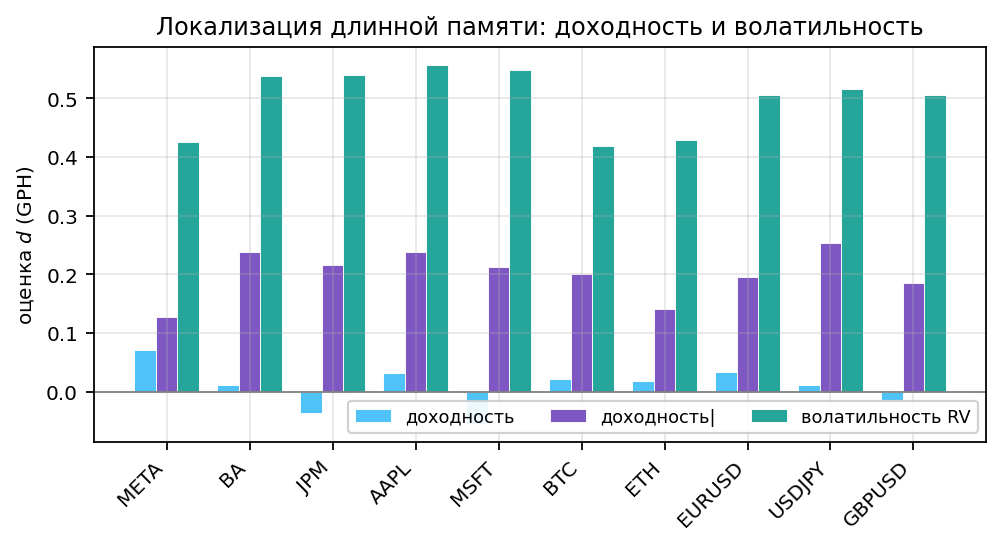
\includegraphics[width=\columnwidth]{fig_memory_localization.png}
\caption{Localisation of long memory. GPH estimates of the fractional integration parameter $d$ for
logarithmic returns, absolute returns and realised volatility, by asset.}
\label{fig:loc}
\end{figure}
\begin{table}[H]
\centering\small
\caption{Local memory of realised volatility: mean estimates over the rolling window ($W=500$), crisis and
calm regimes and significance of the structural break (CUSUM) and of the regime difference (Welch $t$-test).}
\label{tab:mem}
\begin{tabularx}{\columnwidth}{|X|c|c|c|c|c|}
\hline
Asset & $\bar{\hat d}$ & $\hat H$ & crisis & calm & $p_{\mathrm{CUSUM}}$ \\
\hline
META   & 0.426 & 0.897 & 0.386 & 0.446 & $<0.001$ \\
BA     & 0.538 & 0.937 & 0.480 & 0.568 & $<0.001$ \\
JPM    & 0.539 & 0.911 & 0.469 & 0.574 & $<0.001$ \\
AAPL   & 0.556 & 0.951 & 0.472 & 0.598 & 0.003 \\
MSFT   & 0.548 & 0.948 & 0.480 & 0.582 & $<0.001$ \\
BTC    & 0.419 & 0.905 & 0.416 & 0.420 & 0.056 \\
ETH    & 0.430 & 0.912 & 0.443 & 0.424 & 0.448 \\
EURUSD & 0.506 & 0.932 & 0.430 & 0.551 & $<0.001$ \\
USDJPY & 0.516 & 0.915 & 0.458 & 0.550 & $<0.001$ \\
GBPUSD & 0.505 & 0.939 & 0.463 & 0.531 & 0.061 \\
\hline
\end{tabularx}
\end{table}

\subsection{The strength of memory is non-stationary and collapses in crises}

The local estimates are far from constant. Over the sample the range of $\hat d(t)$ reaches half
its own mean for individual assets --- from $0.33$ to $0.75$ for MSFT --- and the CUSUM test
detects a structural shift in the trajectory of $\hat d(t)$ for seven of the ten assets, with
$p$-values below $0.005$ in five cases and below $0.001$ in four. The comparison of crisis and
calm windows is significant for the same seven assets, and the direction is consistent: the mean
local memory falls from $0.52$ in calm periods to $0.45$ in crisis periods, i.e. by
approximately $13\%$.

Figure~\ref{fig:crisis} contrasts the mean local memory in calm and in crisis periods for every asset.
The most pronounced collapse occurs during the 2022 interest-rate tightening cycle, when the local
memory of equities and currency pairs falls synchronously from the $0.65$--$0.75$ range to
$0.30$--$0.45$. Cryptocurrencies constitute the notable exception: for BTC and ETH neither the
CUSUM test nor the regime comparison rejects the null ($p=0.056$ and $p=0.448$ for the CUSUM
test, $p=0.906$ and $p=0.159$ for the Welch test), and the crisis and calm means coincide. This
pattern is consistent with the distinct regime dynamics of crypto markets, which exhibit a
persistent high-frequency component and are less sensitive to the monetary-policy channel.

\begin{figure}[H]
\centering
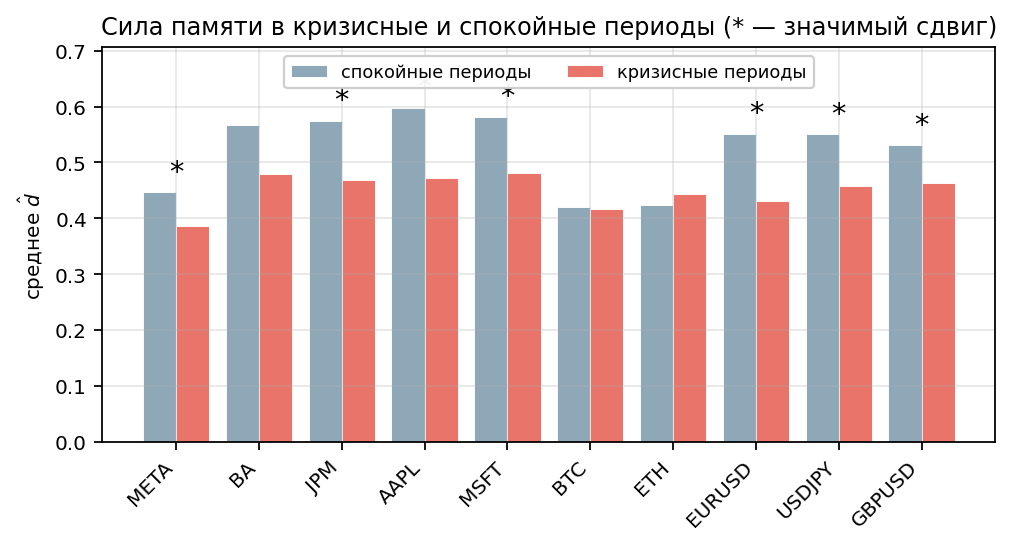
\includegraphics[width=\columnwidth]{fig_crisis.png}
\caption{Mean local memory in calm and in crisis periods. An asterisk marks a significant
difference between the two regimes (Welch $t$-test).}
\label{fig:crisis}
\end{figure}

\begin{figure}[H]
\centering
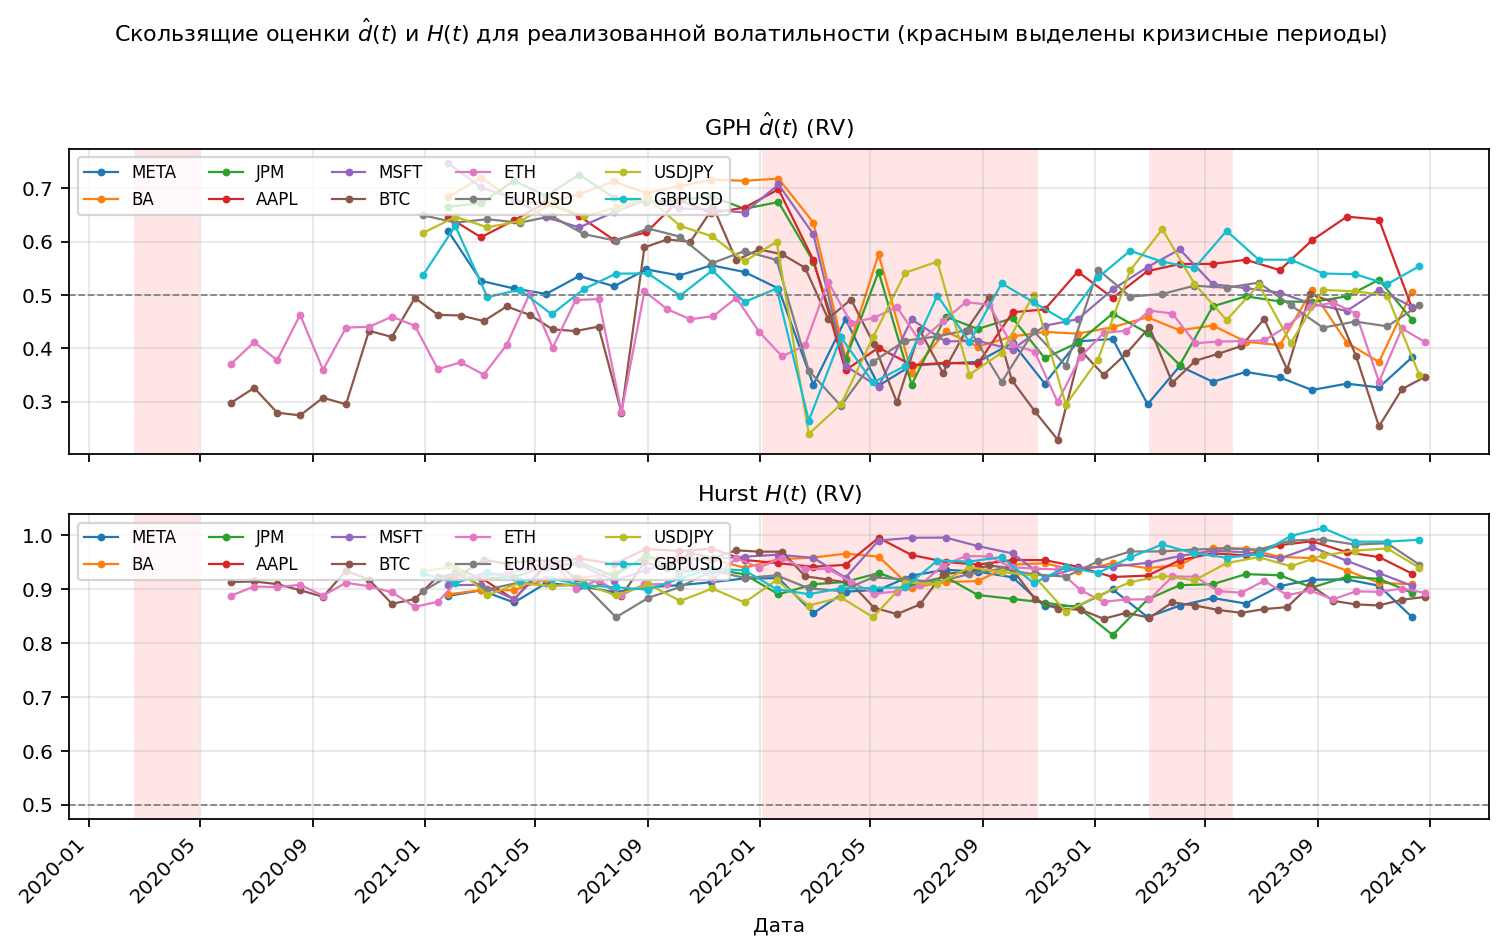
\includegraphics[width=\columnwidth]{paper_memory.png}
\caption{Rolling estimates $\hat d(t)$ and $H(t)$ for realised volatility; crisis periods are highlighted.}
\label{fig:mem}
\end{figure}

\subsection{The local memory estimate improves volatility forecasts}

Adding the local memory features $\hat d_t$ and $\Delta\hat d_t$ to HAR-RV improves the
out-of-sample forecast for all ten assets in terms of MSE, with an average gain of $+7.1\%$, and
for eight of the ten assets in terms of QLIKE, with an average gain of $+1.8\%$. The gains are
concentrated in the volatile instruments: $+26.9\%$ for META and $+16.1\%$ for BTC. The two
assets for which the QLIKE gain is negative (MSFT, $-5.7\%$; GBPUSD, $-0.3\%$) still exhibit
positive MSE gains, which indicates that the memory features improve the point forecast but can
occasionally shift the estimated conditional distribution towards the tails. Figure~\ref{fig:har}
displays the gains asset by asset.

\begin{figure}[H]
\centering
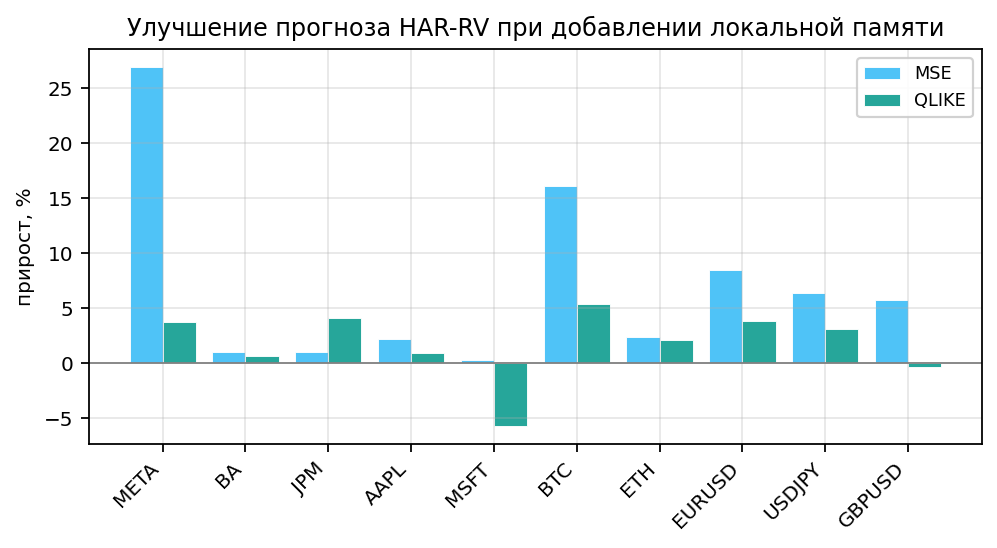
\includegraphics[width=\columnwidth]{fig_har_improvement.png}
\caption{Improvement of the HAR-RV forecast after adding the local memory features $\hat d_t$ and
$\Delta\hat d_t$, in per cent, by asset and by loss function.}
\label{fig:har}
\end{figure}

\begin{table}[H]
\centering\small
\caption{Improvement of HAR-RV after adding the local memory features $\hat d_t$ and $\Delta\hat d_t$
(expanding-window estimation, 2019--2023).}
\label{tab:har}
\begin{tabularx}{\columnwidth}{|X|c|c|}
\hline
Asset & $\Delta$MSE, \% & $\Delta$QLIKE, \% \\
\hline
META   & $+26.9$ & $+3.8$ \\
BA     & $+1.0$  & $+0.6$ \\
JPM    & $+1.0$  & $+4.1$ \\
AAPL   & $+2.2$  & $+0.9$ \\
MSFT   & $+0.3$  & $-5.7$ \\
BTC    & $+16.1$ & $+5.4$ \\
ETH    & $+2.4$  & $+2.1$ \\
EURUSD & $+8.5$  & $+3.8$ \\
USDJPY & $+6.4$  & $+3.1$ \\
GBPUSD & $+5.8$  & $-0.3$ \\
\hline
\end{tabularx}
\end{table}

\subsection{Static attention mechanisms degrade differently across memory regimes}

All three attention mechanisms degrade when the memory regime switches from low to high, but they
do so to very different degrees (Table~\ref{tab:attn}). Full self-attention loses $+51\%$ in RMSE,
the two-path MultiFeature mechanism $+50\%$, and the sparse ProbSparse mechanism $+143\%$: under
strong memory the top-$k$ selection discards informative long-range links and the model collapses.
MultiFeature is the most stable mechanism in both regimes, which suggests that the decomposition of
the representation across scales is more important for long-memory series than the raw sparsity of
the attention map. No static mechanism is optimal in both regimes, which is the quantitative
justification for the adaptive design of Section~\ref{sec:memadapt}. Figure~\ref{fig:attn}
illustrates the effect for the three mechanisms.

\begin{figure}[H]
\centering
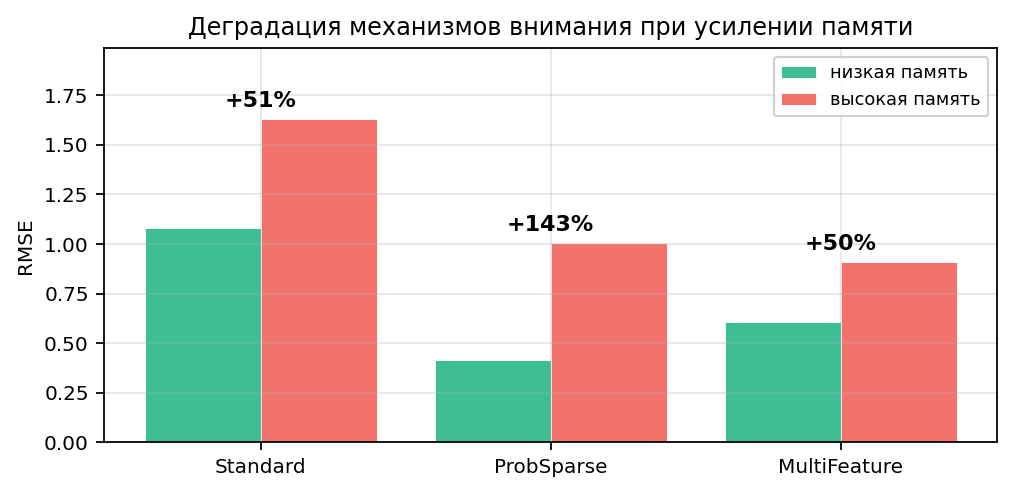
\includegraphics[width=\columnwidth]{fig_attention_deg.png}
\caption{Degradation of the attention mechanisms across memory regimes: RMSE in the low-memory and
in the high-memory regime, with the relative growth indicated.}
\label{fig:attn}
\end{figure}

\begin{table}[H]
\centering\small
\caption{RMSE of the attention mechanisms in the low- and high-memory regimes and its relative growth.}
\label{tab:attn}
\begin{tabularx}{\columnwidth}{|X|c|c|c|}
\hline
Mechanism & low memory & high memory & growth, \% \\
\hline
Standard    & 1.078 & 1.628 & $+51$ \\
ProbSparse  & 0.415 & 1.006 & $+143$ \\
MultiFeature & 0.608 & 0.911 & $+50$ \\
\hline
\end{tabularx}
\end{table}

% ======= 6. Discussion =======

\section{Discussion}\label{sec:discussion}

\subsection{Interpretation}

Taken together, the three experiments support a single conclusion: the long-term memory of
volatility is not a static property of the series but a dynamic one, and this dynamics carries
usable information. Three implications follow.

First, the classical econometric models are mis-specified in a specific, measurable way. The
damage is not diffuse but concentrated: the fixed memory structure produces its largest errors
exactly at regime changes, which are the periods in which risk measurement matters most.

Second, the transformer reading of attention as a learnable autocorrelation function is
substantive, not merely metaphorical, and it carries a design consequence. An attention scheme that
does not depend on the estimated memory cannot be optimal across regimes --- and this is
confirmed quantitatively, since the degradation is not uniform across mechanisms but depends
precisely on how the mechanism treats long-range links.

Third, the predictive content of the local memory estimate is economically meaningful. A
$7.1\%$ average reduction in the mean-squared error of a benchmark model, obtained by adding two
regressors, is not a marginal improvement; and it is obtained without any change to the
forecasting model itself.

\subsection{Limitations and the critique of long-memory diagnostics}

The results must be interpreted in the light of the critique developed by Gatheral, Jaisson and
Rosenbaum [12]. Their analysis shows that the log-volatility of equity indices
behaves essentially as a fractional Brownian motion with $H$ of order $0.1$, and that classical
long-memory diagnostics --- the scaling of the integrated variance, the behaviour of
fractionally differentiated series --- then produce a spurious long-memory conclusion. If a
comparable mechanism operates in realised volatility, the interpretation of $\hat d$ as a
structural parameter of the data-generating process is not warranted, and the estimates reported
here should be viewed as \emph{local diagnostics of persistence} rather than as estimates of a
true fractional integration parameter.

This limitation does not invalidate the present findings, but it does change their interpretation,
and we prefer to state this explicitly. The object of study here is the \emph{time variation} of
the local estimate. A quantity that is not a structural parameter of the process may still be
informative about the state of the market, exactly as a moving average of volatility is
informative about the level of volatility without being a parameter of any model. The gains in
forecast accuracy reported in Section~\ref{sec:results} are estimated out of sample against a
fixed benchmark and are therefore not explained by the mere presence of a persistent regressor.

Three further limitations should be mentioned. The sample covers a single five-year window that
contains the COVID-19 shock but not a longer sequence of independent crises, so the regime
statistics are based on a moderate number of events. The pilot experiment on attention mechanisms
uses minute-frequency data on a limited set of assets and serves to demonstrate the phenomenon
rather than to establish its magnitude. Finally, the proposed Memory-Adaptive Attention mechanism
has been formulated and its technical prerequisites identified, but a full implementation with an
embedded differentiable estimator remains the subject of subsequent work; the present paper
establishes the problem, the diagnostic evidence and the design principle.

\subsection{Research outlook}

The programme that follows from the present results has three components: a mathematical
formalisation of the adaptive mechanism, including the relation between the structure of attention
and the autocovariance function of fractionally integrated processes; the implementation of a
differentiable local memory estimator embedded in the architecture; and an extension of the
evaluation to a full comparison with econometric and neural baselines, culminating in the
construction and backtesting of VaR and ES estimates on the basis of the improved forecasts.

% ======= 7. Conclusion =======

\section{Conclusion}\label{sec:concl}

The paper has investigated the non-stationarity of long-term memory in the volatility of financial
time series and its predictive value, and has examined the consequences of this phenomenon for
the design of attention mechanisms. The empirical evidence, obtained on a sample of ten assets from
three asset classes over 2019--2023, is unambiguous on three points. Long-term memory in
volatility is strong and is clearly stronger than in returns: $\hat d$ of the order of $0.42$--$0.56$
against values indistinguishable from zero for logarithmic returns. The strength of this memory is
significantly non-stationary for seven of the ten assets, and it weakens systematically in crisis
periods, the mean local estimate falling from $0.52$ to $0.45$. And the local memory estimate
carries independent forecasting information, improving HAR-RV by $+7.1\%$ in MSE on average and by
$+1.8\%$ in QLIKE for eight of the ten assets.

These results have a direct methodological consequence. Because the self-attention mechanism is a
learnable autocorrelation function, and because the attention schemes currently used in the
state-of-the-art long-horizon architectures are specified a priori, no static scheme can be optimal
across memory regimes; the quantitative degradation reported here --- from $+50\%$ for the
most robust mechanism to $+143\%$ for the sparsest --- demonstrates the size of the effect that an
adaptive mechanism would have to capture. The Memory-Adaptive Attention construction proposed
above, in which a differentiable local memory estimator controls the effective context length and
the sparsity of attention, together with the recent results on differentiable estimation of the
Hurst and fractional integration parameters, provides a technically feasible route to closing this
gap.

\ListReferences{
\item Andersen, T.~G., Bollerslev, T., Diebold, F.~X., Labys, P. Modeling and forecasting realized volatility. \textit{Econometrica}, 2009, vol.~71, no.~2, pp.~579--625.
\item Baillie, R.~T., Bollerslev, T., Mikkelsen, H.~O. Fractionally integrated generalized autoregressive conditional heteroskedasticity. \textit{Journal of Econometrics}, 1996, vol.~74, no.~1, pp.~3--30.
\item Banerjee, A., Urga, G. Modelling structural breaks, long memory and stock market volatility: an overview. \textit{Journal of Econometrics}, 2005, vol.~129, no.~1--2, pp.~1--34.
\item Beran, J. \textit{Statistics for Long-Memory Processes}. Chapman \& Hall/CRC, 1994.
\item Boros, D. et al. Deep learning the Hurst parameter of linear fractional processes and assessing its reliability. arXiv:2401.01789, 2024.
\item Choi, K., Yu, W.-C., Zivot, E. Long memory versus structural breaks in modeling and forecasting realized volatility. \textit{Journal of International Money and Finance}, 2010, vol.~29, no.~5, pp.~857--875.
\item Christoffersen, P.~F. Evaluating interval forecasts. \textit{International Economic Review}, 1998, vol.~39, no.~4, pp.~841--862.
\item Corsi, F. A simple approximate long-memory model of realized volatility. \textit{Journal of Financial Econometrics}, 2009, vol.~7, no.~2, pp.~174--196.
\item Csan\'ady, B. et al. Parameter estimation of long memory stochastic processes with deep neural networks. arXiv:2410.03776, 2024.
\item Di Persio, L., Russo, M. Deep neural network model for Hurst exponent: learning from R/S analysis. \textit{Mathematics}, 2024, vol.~12, no.~22, art.~3483.
\item Ding, Z., Granger, C.~W.~J., Engle, R.~F. A long memory property of stock market prices and a new model. \textit{Journal of Empirical Finance}, 1993, vol.~1, no.~1, pp.~1--28.
\item Gatheral, J., Jaisson, T., Rosenbaum, M. Volatility is rough. \textit{Quantitative Finance}, 2018, vol.~18, no.~6, pp.~933--949.
\item Geweke, J., Porter-Hudak, S. The estimation and application of long memory time series models. \textit{Journal of Time Series Analysis}, 1983, vol.~4, no.~4, pp.~221--238.
\item Granger, C.~W.~J., Joyeux, R. An introduction to long-memory time series models and fractional differencing. \textit{Journal of Time Series Analysis}, 1980, vol.~1, no.~1, pp.~15--29.
\item Hosking, J.~R.~M. Fractional differencing. \textit{Biometrika}, 1981, vol.~68, no.~1, pp.~165--176.
\item Hurst, H.~E. Long-term storage capacity of reservoirs. \textit{Transactions of the American Society of Civil Engineers}, 1951, vol.~116, no.~1, pp.~770--799.
\item Kupiec, P.~H. Techniques for verifying the accuracy of risk measurement models. \textit{The Journal of Derivatives}, 1995, vol.~3, no.~2, pp.~73--84.
\item Liu, Y. et al. Autoregressive moving-average attention mechanism for time series forecasting. arXiv:2410.03159, 2024.
\item Lo, A.~W. Long-term memory in stock market prices. \textit{Econometrica}, 1991, vol.~59, no.~5, pp.~1279--1313.
\item Makarava, N. et al. Differentiable neural network layer for estimating Hurst and anomalous diffusion exponents. \textit{Journal of Physics A: Mathematical and Theoretical}, 2025, vol.~58, art.~265002.
\item Mandelbrot, B.~B., Van Ness, J.~W. Fractional Brownian motions, fractional noises and applications. \textit{SIAM Review}, 1968, vol.~10, no.~4, pp.~422--437.
\item Mikosch, T., Starica, C. Non-stationarities in financial time series, the long-range dependence, and the IGARCH effects. \textit{The Review of Economics and Statistics}, 2004, vol.~86, no.~1, pp.~378--390.
\item Nie, Y. et al. A time series is worth 64 words: long-term forecasting with transformers. \textit{ICLR}, 2023.
\item Palma, W. \textit{Long-Memory Time Series: Theory and Methods}. John Wiley \& Sons, 2007.
\item Patton, A.~J. Volatility forecast comparison using imperfect volatility proxies. \textit{Journal of Econometrics}, 2011, vol.~160, no.~1, pp.~246--256.
\item Philipper, C. et al. An adaptive temporal attention mechanism to address distribution shifts. \textit{ICLR 2024 Workshop on Agents and Tools for Multi-Task Learning}, 2024.
\item Pipiras, V., Taqqu, M.~S. \textit{Long-Range Dependence and Self-Similarity}. Cambridge University Press, 2017.
\item Tay, Y. et al. Efficient transformers: a survey. \textit{ACM Computing Surveys}, 2022, vol.~55, no.~6, pp.~1--28.
\item Vaswani, A. et al. Attention is all you need. \textit{Advances in Neural Information Processing Systems}, 2017, vol.~30, pp.~5998--6008.
\item Vogl, M. Hurst exponent dynamics of S\&P 500 returns: implications for market efficiency, long memory, multifractality and financial crises predictability. \textit{Chaos, Solitons \& Fractals}, 2023, vol.~166, art.~112884.
\item Wen, Q. et al. Transformers in time series: a survey. \textit{IJCAI}, 2023, pp.~4584--4592.
\item Wu, H. et al. Autoformer: decomposition transformers with auto-correlation for long-term series forecasting. \textit{Advances in Neural Information Processing Systems}, 2021, vol.~34, pp.~22419--22430.
\item Zhang, Z. et al. Twilight: adaptive attention sparsity with hierarchical top-p pruning. arXiv:2502.02770, 2025.
\item Zhou, H. et al. Informer: beyond efficient transformer for long sequence time-series forecasting. \textit{AAAI}, 2021, vol.~35, no.~12, pp.~11106--11115.
\item Zhou, T. et al. FEDformer: frequency enhanced decomposed transformer for long-term series forecasting. \textit{ICML}, PMLR, 2022, pp.~27268--27286.
\item Zhou, Z. SDformer: transformer with spectral filter and dynamic attention for multivariate time series long-term forecasting. \textit{IJCAI}, 2024, pp.~5689--5697.
}

\end{multicols}

\end{document}
